\noindent\markforreview
\vspace{1em}

In the given equation, \(c\) is a constant. The equation has infinitely many solutions. What is the value of \(c\)?
\[
18(x+5)=2(x+c)+16x
\]

\vspace{0.75em}

\choicebox{A}{90}
\choicebox{B}{45}
\choicebox{C}{10}
\choicebox{D}{5}

\vspace{2em}
\noindent\markforreview
\vspace{1em}

Hannah and Wyatt are saving money to purchase a car. Hannah saves \(\frac{1}{5}\) of her salary each month, and Wyatt saves \(\frac{2}{7}\) of his salary each month. Together, they save a total of \$3{,}270 from their monthly salaries each month. If \(h\) and \(w\) represent Hannah's and Wyatt's monthly salaries, in dollars, respectively, which equation shows the relationship between \(h\) and \(w\)?

\vspace{0.75em}

\choicebox{A}{$h+w=3{,}270$}
\choicebox{B}{$h+2w=3{,}270$}
\choicebox{C}{$10h+7w=114{,}450$}
\choicebox{D}{$7h+10w=114{,}450$}

\newpage
\noindent\markforreview
\vspace{1em}

The figure shows a rectangular pool surrounded by a concrete path that is \(x\) feet (ft) wide on all sides. The pool is \(21\) ft long and \(11\) ft wide. The area of the concrete path is \(144\,\text{ft}^2\). What is the value of \(x\)?

\begin{center}
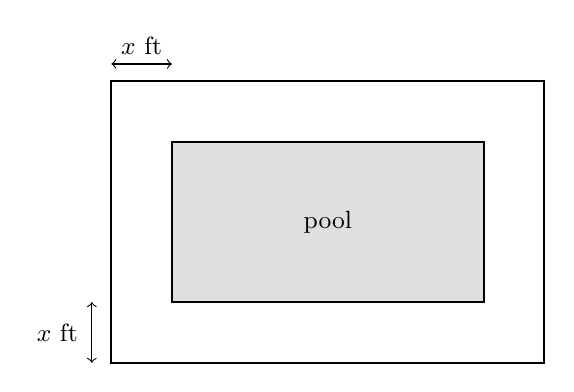
\begin{tikzpicture}[scale=0.55]
  \draw[thick] (0,0) rectangle (10,6.5);
  \fill[gray!25] (1.4,1.4) rectangle (8.6,5.1);
  \draw[thick] (1.4,1.4) rectangle (8.6,5.1);
  \node at (5,3.25) {\small pool};
  \draw[<->] (-0.45,1.4) -- (-0.45,0);
  \node[left] at (-0.55,0.7) {\small \(x\) ft};
  \draw[<->] (1.4,6.9) -- (0,6.9);
  \node[above] at (0.7,6.9) {\small \(x\) ft};
\end{tikzpicture}\\[0.2em]
\textit{Note: Figure not drawn to scale.}
\end{center}

\vspace{0.5em}

\choicebox{A}{2}
\choicebox{B}{4}
\choicebox{C}{18}
\choicebox{D}{36}

\vspace{2em}
\noindent\markforreview
\vspace{1em}

A wildlife biologist counted bald eagles at a nature preserve every day for 21 days. The results are shown in the table below as data set A.

\begin{center}
\begin{tabular}{|c|c|}
\hline
\textbf{Number of bald eagles} & \textbf{Number of days}\\
\hline
0 & 1\\
1 & 3\\
2 & 4\\
3 & 5\\
4 & 4\\
5 & 3\\
19 & 1\\
\hline
\end{tabular}
\end{center}

The value 19 was recorded in error and is removed from data set A to create data set B. Which of the following best compares the median of data set A and the median of data set B?

\vspace{0.75em}

\choicebox{A}{The median of data set B is less than the median of data set A.}
\choicebox{B}{The median of data set B is equal to the median of data set A.}
\choicebox{C}{The median of data set B is greater than the median of data set A.}
\choicebox{D}{There is not enough information to compare the medians of the two data sets.}

\newpage
\noindent\markforreview
\vspace{1em}

The equation \(3x - 9 = 12\) is true for which value of \(x\)?

\vspace{0.75em}

\choicebox{A}{$1$}
\choicebox{B}{$5$}
\choicebox{C}{$7$}
\choicebox{D}{$21$}

\vspace{2em}
\noindent\markforreview
\vspace{1em}

\[
f(x)=4^{-5(x+1)}
\]
Which of the following equivalent forms of the given function \(f\) displays, as the base or the coefficient, the \(y\)-coordinate of the \(y\)-intercept of the graph of \(y=f(x)\) in the \(xy\)-plane?

\vspace{0.75em}

\choicebox{A}{$f(x)=\dfrac{1}{1{,}024}\left(\dfrac{1}{4}\right)^{5x}$}
\choicebox{B}{$f(x)=\left(\dfrac{1}{4}\right)^{5x+5}$}
\choicebox{C}{$f(x)=4^{-5x-5}$}
\choicebox{D}{$f(x)=1{,}024^{-x-1}$}

\noindent\markforreview
\vspace{1em}
\vspace{1em}

One of the equations in a system of two linear equations is given:  
\[
31(x - n) = 31y + 31n
\]  
where \(n\) is a positive constant.  
The system has no solution. Which equation could be the second equation in this system?

\vspace{0.75em}

\choicebox{A}{$3x - 3y = 6n$}
\choicebox{B}{$3x + 3y = 3n$}
\choicebox{C}{$3x + 3y = 6n$}
\choicebox{D}{$3x - 3y = 3n$}

\vspace{2em}

\newpage

\noindent\markforreview
\vspace{1em}
\vspace{1em}

The given equation is one equation in a system of two linear equations.  
If the system of equations has at least one solution, which of the following equations could be the other equation in the system?

\[
7x + 5y = 2
\]

\begin{itemize}
    \item[I.] \(10.5x + 7.5y = 3\)
    \item[II.] \(10.5x - 7.5y = 3\)
\end{itemize}

\choicebox{A}{I only}  
\choicebox{B}{II only}  
\choicebox{C}{I and II}  
\choicebox{D}{Neither I nor II}


\vspace{2em}

\noindent\markforreview
\vspace{1em}
\vspace{1em}

For each real number \( r \), which of the following points lies on the graph of each equation in the \( xy \)-plane for the given system?
\[
\begin{aligned}
2x + 3y &= 7 \\
10x + 15y &= 35
\end{aligned}
\]

\vspace{0.75em}

\choicebox{A}{$\left(\frac{7}{5} + r, -\frac{7}{5} + 35 \right)$}
\choicebox{B}{$\left(-\frac{3r}{2} + \frac{7}{2}, r \right)$}
\choicebox{C}{$\left(r, \frac{2r}{3} + \frac{7}{3} \right)$}
\choicebox{D}{$\left(r, -\frac{3r}{2} + \frac{7}{2} \right)$}


\vspace{2em}

\newpage

\noindent\markforreview
\vspace{1em}
\vspace{1em}

In the \(xy\)-plane, the graph of the linear function \(f\) has a negative slope
and a \(y\)-intercept at \((0,k)\), where \(k\) is a positive constant. Which of
the following must be true?
\[
\begin{array}{ll}
\text{I.} & \text{If }a>b,\text{ then }f(a)<f(b).\\
\text{II.} & \text{If }a<0,\text{ then }f(a)>k.\\
\text{III.} & \text{If }a>0,\text{ then }f(a)>0.
\end{array}
\]
\choicebox{A}{I and II only}
\choicebox{B}{I and III only}
\choicebox{C}{II and III only}
\choicebox{D}{I, II, and III}

\vspace{2em}

\noindent\markforreview
\vspace{1em}
\vspace{1em}

In the \(xy\)-plane, what is the slope of the line that passes through the points \((1,2)\) and \((5,10)\)?

\vspace{0.75em}

\choicebox{A}{$1$}
\choicebox{B}{$2$}
\choicebox{C}{$4$}
\choicebox{D}{$8$}

\newpage

\newpage

\noindent\markforreview
\vspace{1em}
\vspace{1em}

The function $f$ is defined by the given equation: 
\[
f(x) = x^2 - 4x - 320
\]
Which of the following equivalent forms of the equation displays the minimum value of the function as a constant or coefficient?

\vspace{0.75em}

\choicebox{A}{$f(x) = x^2 - 4(x + 80)$}
\choicebox{B}{$f(x) = (x - 2)^2 + (-324)$}
\choicebox{C}{$f(x) = x(x - 4) + (-320)$}
\choicebox{D}{$f(x) = (x + 16)(x - 20)$}

\vspace{2em}
\newpage

\noindent\markforreview
\vspace{1em}
\vspace{1em}

At different times on a certain day, a manager at a theme park recorded the number of visitors.  
An exponential model gives the estimated number of visitors, $V$, at the theme park $t$ hours after the theme park opened, where $t \leq 3$.  
Based on the model, 80 visitors were estimated to be at the theme park when it opened,  
and every 30 minutes the estimated number of visitors increased by 150\% of the number 30 minutes earlier.  
Which of the following equations best represents this model?

\vspace{0.75em}

\choicebox{A}{$V = 80(2.5)^{2t}$}
\choicebox{B}{$V = 80(2.5)^{\frac{t}{30}}$}
\choicebox{C}{$V = 80(1.5)^{2t}$}
\choicebox{D}{$V = 80(1.5)^{\frac{t}{30}}$}

\vspace{2em}
\newpage

\newpage

\noindent\markforreview
\vspace{1em}
\vspace{1em}

An economist fits a quadratic revenue model \(y = f(x)\) that breaks even at two production levels. The function \(f\) is defined by
\[
f(x) = ax^2 + bx + c,
\]
where \(a, b, c\) are constants. The graph of \(y = f(x)\) passes through the points \((9, 0)\) and \((-2, 0)\). If \(a\) is an integer greater than 1, which of the following could be the value of \(a + b\)?

\vspace{0.75em}

\choicebox{A}{\(8\)}
\choicebox{B}{\(7\)}
\choicebox{C}{\(-6\)}
\choicebox{D}{\(-12\)}

\vspace{2em}
\newpage

\noindent\markforreview
\vspace{1em}
\vspace{1em}

A savings balance is modeled by an exponential function of time. In the given function, \(b\) is a positive constant. For every increase in the value of \(x\) by 1, the value of \(f(x)\) increases by \(c\%\), where \(0 < c < 100\).

Which expression gives the value of \(c\) in terms of \(b\)?
\[
f(x) = 66(b)^x
\]

\vspace{0.75em}

\choicebox{A}{\(1 + \dfrac{b}{100}\)}
\choicebox{B}{\(b + 100\)}
\choicebox{C}{\(100(b + 1)\)}
\choicebox{D}{\(100(b - 1)\)}

\vspace{2em}
\newpage

\newpage

\noindent\markforreview
\vspace{1em}
\vspace{1em}

The exponential function \(f\) is defined by
\[
f(x) = ab^x,
\]
where \(a\) and \(b\) are positive constants.
If \(f(s) = t\) and \(f(s + 1) = t - 0.87t\), where \(s\) and \(t\) are constants, what is the value of \(b\)?

\vspace{0.75em}

\choicebox{A}{0.13}
\choicebox{B}{0.87}
\choicebox{C}{1.13}
\choicebox{D}{1.87}

\vspace{2em}
\newpage

\noindent\markforreview
\vspace{1em}
\vspace{1em}

Let \(f(x) = x^3 - 9x\) and \(g(x) = x^2 - 2x - 3\). Which of the following expressions is equivalent to \(\dfrac{f(x)}{g(x)}\) for \(x > 3\)?

\vspace{0.75em}

\choicebox{A}{$\dfrac{1}{x + 1}$}
\choicebox{B}{$\dfrac{x + 3}{x + 1}$}
\choicebox{C}{$\dfrac{x(x - 3)}{x + 1}$}
\choicebox{D}{$\dfrac{x(x + 3)}{x + 1}$}

\newpage

\newpage

\noindent\markforreview
\vspace{1em}
\vspace{1em}

The function \(f(x) = 4x^2 + 64x + 262\) is defined, and \(g(x) = f(x + 5)\). For what value of \(x\) does \(g(x)\) reach its minimum?

\vspace{0.75em}

\choicebox{A}{$-13$}
\choicebox{B}{$-8$}
\choicebox{C}{$-5$}
\choicebox{D}{$-3$}

\vspace{2em}

\noindent\markforreview
\vspace{1em}
\vspace{1em}

For data set A, the table summarizes the distribution of the number of pieces of mail received by a business each day during a period of 11 days.

\[
\begin{array}{|c|c|}
\hline
\text{Pieces of mail} & \text{Days} \\
\hline
0 & 2 \\
4 & 2 \\
5 & 2 \\
6 & 2 \\
7 & 1 \\
8 & 1 \\
17 & 1 \\
\hline
\end{array}
\]

The data value $17$ is removed from data set A to create data set B, which consists of the remaining 10 data values.  
Which statement best compares the median of data set A and the median of data set B?

\vspace{0.75em}

\choicebox{A}{The median of data set B is less than the median of data set A.}
\choicebox{B}{The median of data set B is greater than the median of data set A.}
\choicebox{C}{The median of data set B is equal to the median of data set A.}
\choicebox{D}{There is not enough information to compare the medians of the two data sets.}

\vspace{2em}
\newpage

\newpage

\noindent\markforreview
\vspace{1em}
\vspace{1em}

\vspace{1em}

\begin{center}
\begin{tabular}{|c|c|}
\hline
\textbf{Data} & \textbf{Frequency}\\
\hline
1 & 2\\
2 & 5\\
3 & 6\\
4 & 5\\
5 & 2\\
\hline
\end{tabular}
\end{center}

The frequency table above summarizes data set A. 
Data set B is created by multiplying all of the values in data set A by $2$. 
Which of the following must be true?

\begin{itemize}
\item[I.] The difference between the mean and median of data set B is $0$.
\item[II.] The standard deviation of data set B is equal to the standard deviation of data set A.
\item[III.] The range of data set B is double the range of data set A.
\end{itemize}

\vspace{0.75em}

\choicebox{A}{I and II only}  
\choicebox{B}{II and III only}  
\choicebox{C}{I and III only}  
\choicebox{D}{I, II, and III}
\newpage

\newpage

\noindent\markforreview
\vspace{1em}
\vspace{1em}

In isosceles triangle $ABC$, sides $AB$ and $AC$ are congruent. Point $D$ divides side $BC$ such that the length of $\overline{BD}$ is $\dfrac{4}{7}$ of the length of $\overline{BC}$. Point $E$ lies on side $AB$ and point $F$ lies on side $AC$ such that when segments $\overline{DE}$ and $\overline{DF}$ are drawn, angle $\angle BED$ is congruent to angle $\angle CFD$. If the length of $\overline{BE}$ is $8$, what is the length of $\overline{CF}$?

\vspace{0.75em}

\choicebox{A}{6}
\choicebox{B}{14}
\choicebox{C}{32}
\choicebox{D}{56}

\vspace{2em}
\newpage

\newpage

\noindent\markforreview
\vspace{1em}
\vspace{1em}

Triangle $ABC$ is similar to triangle $DEF$, where $A$ corresponds to $D$ and $C$ corresponds to $F$.  
Angles $C$ and $F$ are right angles.  
If $\tan(A) = \sqrt{5}$ and $DF = 53$, what is the length of $DE$?

\vspace{0.75em}

\choicebox{A}{$\dfrac{53\sqrt{3}}{5}$}
\choicebox{B}{$\dfrac{53\sqrt{3}}{2}$}
\choicebox{C}{$53\sqrt{6}$}
\choicebox{D}{$106$}

\vspace{2em}
\newpage
